\section{Modeling}
\subsection{Definitions}
\begin{description}
    \item[Technical System] The system that should be controlled by the embedded software
    \item[Technical Process] Is part of a technical system and obeys the laws of physics.
          Has always a specific state and this state is defined by physical measurable values.
    \item[Parallel Technical Processes] Multiple technical processes are parallel, i.e. sequentially independent, if their states are physically independent
    \item[Physical (continuous) State of a Technical Process] The physical measurable quantities of all objects involved in a technical-process at a given time
    \item[Time] Time as global physical quantity
    \item[(Discrete) State (State Classes), Logical State] Not all physical quantities are relevant for the control of a technical-process, i.e., not all physical measurement quantities and not all values
\end{description}

\subsection{Domain Oriented Embedded System Construction (DESC)}
\subsubsection{Correspondence Principle}
The software of an embedded system must correspond to the technical system in structure and behaviour.
Strives for correspondence between:
\begin{table}[h]
    \begin{tabular}{ll}\hline
        Domain                             & Software Model                   \\\hline
        Technical system                   & Model of embedded system         \\
        Technical process                  & Reactive object                  \\
        Event                              & Event message                    \\
        Action                             & Action message                   \\
        State machine of technical process & State machine of reactive object \\\hline
    \end{tabular}
\end{table}

\subsubsection{Formal Model}
\begin{itemize}
    \item Basic requirement for the correspondence principle
    \item Correspondence between programm code and real environment is almost impossible
    \item The semantics of programming languages is not built for a correspondence on this level of abstraction
    \item Abstract, omits irrelevant details (e.g. target hardware, programming language)
    \item Allows complete code generation
\end{itemize}

\paragraph{Graphical Representation}
\begin{itemize}
    \item Graphical views of the model
    \item \glqq One picture says more than thousands of words\grqq
    \item Improve readability
\end{itemize}

\paragraph{Executable and Testable Model}
\begin{itemize}
    \item Executable model of system behaviour
    \item Testable system behaviour
    \item Independent of target hardware
\end{itemize}

\paragraph{Code Generation}
\begin{itemize}
    \item Model and code are always consistent
    \item To enable code generation, model has to be formal and complete
    \item All necessary information is contained in the model, in a machine-readable form
\end{itemize}


\begin{paracol}{2}
    \subsubsection{Component Architecture}
    \begin{itemize}
        \item Model consists of components and connectors
        \item Explicit connectors must be independent elements of a composition
        \item Components have to fulfil the correspondence principle
        \item Components of the real system are represented in the model by corresponding objects (boundary-objects)
    \end{itemize}

    \paragraph{Components}
    \begin{itemize}
        \item Reusable building blocks of a system
        \item Independent from each other
        \item Connected by connectors, belonging to the composition
        \item Separately testable
    \end{itemize}

    \switchcolumn
    \raisebox{-1\height}{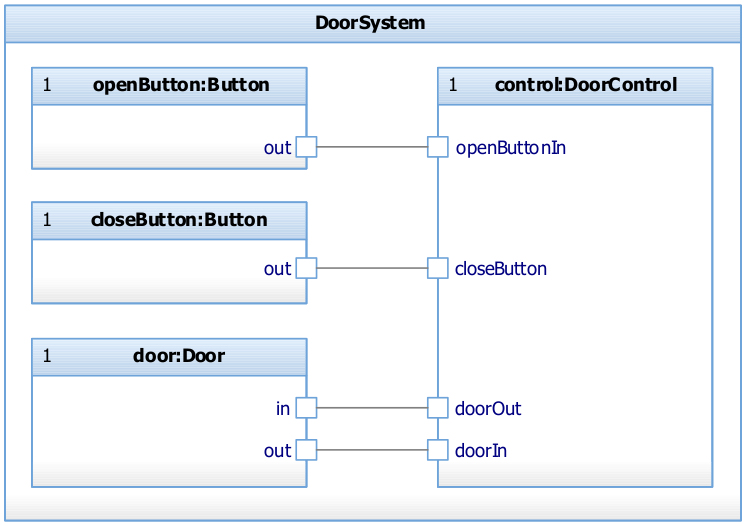
\includegraphics[width=0.49\textwidth]{images/Modeling/component_architecture.png}}
\end{paracol}


\subsubsection{Separation of Concerns}
Embedded system development can be divided into three essential problem areas
\begin{itemize}
    \item Control Software (Control)
          \begin{itemize}
              \item Realisation of the functional requirements
              \item Depends only on the functional requirements and the technical processes
          \end{itemize}
    \item Connection Software (Connection)
          \begin{itemize}
              \item Connection between control software and technical processes
              \item Implements the virtual interaction
          \end{itemize}
    \item Execution Software (Execution)
          \begin{itemize}
              \item Control and connection software are passive parts of the embedded system
              \item Execution software is the active part of the embedded system software
              \item Activates control and connection
              \item Is responsible for meeting the timing requirements
          \end{itemize}
\end{itemize}

\subsection{Generic Software Architecture}
The separation of concerns leads to a generic software architecture for embedded-systems.

{\color{red}red = Control}, {\color{blue}blue=Connection}, {\color{green}green = Execution}

\textbf{Advantages}
\begin{itemize}
    \item Reactive machine and connection independent from each other $\rightarrow$ enables parallel development
    \item Reactive machine is hardware independent
          \begin{itemize}
              \item If the hardware changes, only connection must be changed
              \item Can be simulated and tested on host
              \item Reuse of intellectual property
          \end{itemize}
\end{itemize}

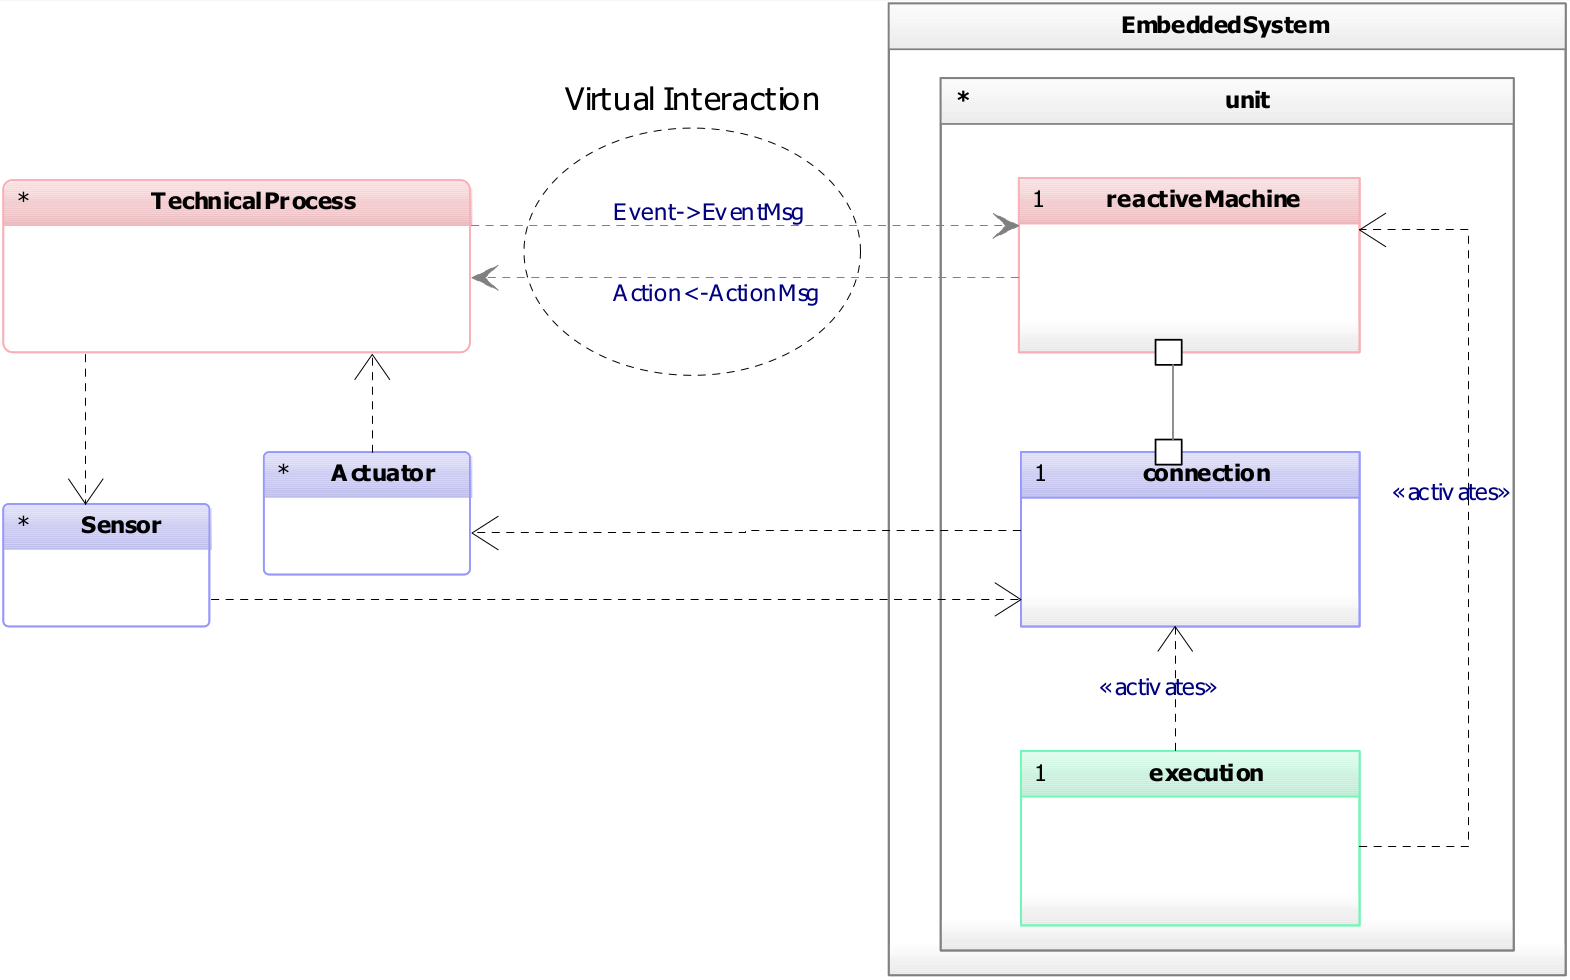
\includegraphics[width=1\textwidth]{images/Modeling/generic_software_architecture.png}

\subsubsection{Control}
\begin{itemize}
    \item Reactive behaviour model
    \item Reacts to input and generates output
    \item Input = Event-Messages, Output = Action-Messages
\end{itemize}

\paragraph{Run-to-Completion}
\begin{itemize}
    \item Reactive-Machine (RM) works sequentially
    \item Events are handled one-at-a-time
    \item Handling of an event cannot be interrupted by other event messages
    \item This non interruptible handling of events is called Run-to-Completion
    \item $\rightarrow$ processes asynchronously arriving messages in a sequential order
\end{itemize}

\paragraph{Reactive Machine}
\begin{itemize}
    \item The reactive-machine is modelled as a collection of reactive-clusters
    \item Each reactive-cluster is a composition of cooperating reactive-objects
    \item Each reactive-object has its own state-machine
\end{itemize}

\paragraph{Virtual Interaction}
\begin{itemize}
    \item Concept of abstraction
    \item A virtual, imaginary, not really existing interaction between technical process and embedded system, respective
\end{itemize}

\paragraph{Correspondence}
\begin{description}
    \item[Event $\rightarrow$ Event Message] In a technical process an event occurs, the reactive machine receives an equally named event message.
          An event message may contain additional attribute values
    \item[Action $\leftarrow$ Action Message] Every action message sent by the embedded system, results in an action applied to the technical process.
\end{description}

\paragraph{Transmission Sequence of (Event) Messages}
\begin{itemize}
    \item Messages of one (sequential) technical process can only arrive one after another
    \item Messages of different technical processes may arrive simultaneously
    \item Messages from one technical process are transmitted strictly in sequential order
    \item Messages can pass messages of other technical processes
\end{itemize}

\subsubsection{Connection}
\begin{itemize}
    \item Implementation of the virtual interaction
    \item Reads input-signals from ports or any other interface
    \item Detects events
    \item Generates event messages
    \item Writes event messages into a message buffer (e.g. queue)
    \item Generates output
    \item Translates action messages into output signals
\end{itemize}

\columnratio{0.5}
\begin{paracol}{2}
    \subsubsection{Execution}
    \begin{itemize}
        \item Controls the sequence of activation of the passive parts of the unit
        \item Responsible for:
              \begin{itemize}
                  \item Activation of the passive parts, i.e. connection and reactive machine
                  \item Management of input- and output-message buffer (queue)
                  \item Scheduling within the Unit, i.e. when to handle which event
              \end{itemize}
        \item Will the input-queue be emptied, before the embedded connection is activated again, or is there a certain abort criterion?
        \item Abort criterion for the cycle
        \item Depends on:
              \begin{itemize}
                  \item Specified reaction times, deadlines
                  \item Execution times of connection and reactive machine $\rightarrow$ can therefore only be implemented at the end, i.e. when the other parts are finished
              \end{itemize}
    \end{itemize}

    \switchcolumn

    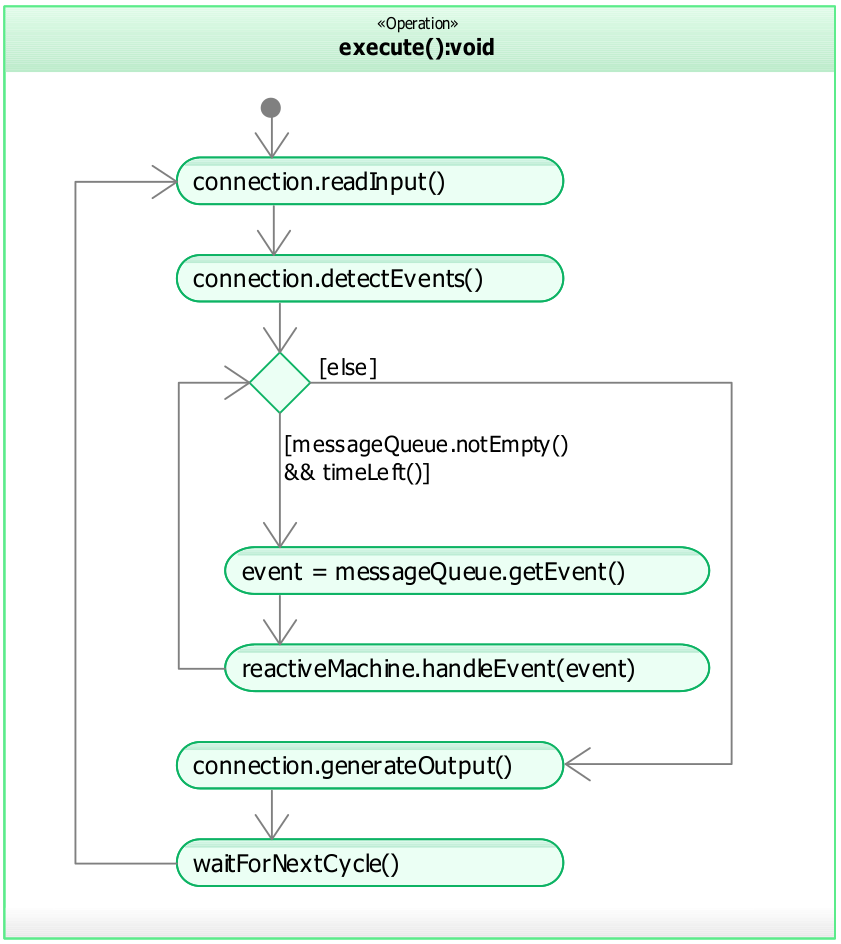
\includegraphics[width=0.49\textwidth]{images/Modeling/execute.png}
\end{paracol}

\subsection{More than one Unit}
\subsubsection{Distributed System}
Distribution on more than one processor nodes
\begin{itemize}
    \item Local distribution of a system
    \item High computing power required
    \item Strict functional separation due to security reasons
\end{itemize}

\subsubsection{On a single Processor}
\paragraph{Modularity}
\begin{itemize}
    \item Concurrent units on a single processor
    \item Required modularity and isolation of parts of the system due to security or other reasons …
\end{itemize}

\paragraph{Different Categories of Response Times}
\begin{itemize}
    \item Different reaction times for different control functions $\rightarrow$ Response time category
    \item One unit per Response Time Category
    \item Fast units may pre-empt slower ones (preemptive scheduling)
    \item Units e.g. as tasks in an RTOS (Real-time Operating System)
\end{itemize}